\documentclass{article}
\usepackage{amsmath, amssymb}
\usepackage{tikz}
\usetikzlibrary{positioning, arrows.meta}


\begin{document}

\title{DNA Matching using STR and Interactive Zero Knowledge Proofs}
\author{Your Name}
\maketitle

\section{Problem Statement}
We aim to design a protocol for DNA matching using Short Tandem Repeats (STR) analysis while preserving privacy through Zero Knowledge Proofs (ZKPs).

\section{Definitions}

\begin{align*}
    &\text{DNA}_A, \text{DNA}_B: \text{DNA sequences of Alice and Bob} \\
    &\text{STR}_A, \text{STR}_B: \text{STR profiles of Alice and Bob} \\
    &S_A, S_B: \text{Secret keys of Alice and Bob} \\
    &R_A, R_B: \text{Random values generated by Alice and Bob} \\
    &H(\cdot): \text{Cryptographic hash function} \\
    &ZKP(\cdot): \text{Zero Knowledge Proof protocol} \\
    &\langle x \rangle_{S_A}: \text{ElGamal encryption of $x$ using Alice's secret key} \\
    &\langle x \rangle_{S_B}: \text{ElGamal encryption of $x$ using Bob's secret key}
\end{align*}

\section{Protocol}

\subsection{Setup}

\begin{enumerate}
    \item Alice and Bob agree on a set of specific STR loci to analyze.
    \item Both Alice and Bob generate their STR profiles, $\text{STR}_A$ and $\text{STR}_B$, from their DNA sequences.
    \item Alice and Bob share the list of selected STR loci.
    \item Alice and Bob each generate a random value: $R_A$ and $R_B$, respectively.
\end{enumerate}

\subsection{Zero Knowledge Proof (ZKP)}

\begin{enumerate}
    \item Alice and Bob interactively prove the equality of their STR profiles without revealing the actual values.
    \item In each iteration $i$:
        \begin{enumerate}
            \item Alice commits to her STR value at locus $i$:
                \[ C_{A,i} = H(\text{STR}_{A,i} || R_{A,i}) \]
            \item Bob commits to his STR value at locus $i$:
                \[ C_{B,i} = H(\text{STR}_{B,i} || R_{B,i}) \]
            \item Alice sends $C_{A,i}$ to Bob, and Bob sends $C_{B,i}$ to Alice.
            \item Alice challenges Bob to prove knowledge of $\text{STR}_{B,i}$:
                \[ \text{ZKP}(C_{B,i}, \text{STR}_{B,i}) \]
            \item Bob challenges Alice to prove knowledge of $\text{STR}_{A,i}$:
                \[ \text{ZKP}(C_{A,i}, \text{STR}_{A,i}) \]
            \item Both proofs are verified using ZKP verification.
        \end{enumerate}
    \item This process is repeated for all selected STR loci.
\end{enumerate}

\section{Verification}

\begin{enumerate}
    \item After completing the Zero Knowledge Proof protocol for all selected STR loci, Alice and Bob can be reasonably confident that their STR profiles match without disclosing any specific genetic information.
\end{enumerate}

\subsection{Schematic}


\begin{align*}
    &\text{DNA}_{\text{POI}}, \text{DNA}_{\text{Police}}: \text{DNA sequences of the Person of Interest and Police} \\
    &\text{STR}_{\text{POI}}, \text{STR}_{\text{Police}}: \text{STR profiles of the Person of Interest and Police} \\
    &S_{\text{POI}}, S_{\text{Police}}: \text{Secret keys of the Person of Interest and Police} \\
    &R_{\text{POI}}, R_{\text{Police}}: \text{Random values generated by the Person of Interest and Police} \\
    &H(\cdot): \text{Cryptographic hash function} \\
    &ZKP(\cdot): \text{Zero Knowledge Proof protocol} \\
    &\langle x \rangle_{S_{\text{POI}}}: \text{ElGamal encryption of $x$ using the Person of Interest's secret key} \\
    &\langle x \rangle_{S_{\text{Police}}}: \text{ElGamal encryption of $x$ using the Police's secret key}
\end{align*}

\section{Protocol}

\subsection{Setup}

\begin{enumerate}
    \item The Police and Person of Interest agree on a set of specific STR loci to analyze.
    \item Both parties generate their STR profiles, $\text{STR}_{\text{POI}}$ and $\text{STR}_{\text{Police}}$, from their DNA sequences.
    \item The Police and Person of Interest share the list of selected STR loci.
    \item The Police and Person of Interest each generate a random value: $R_{\text{POI}}$ and $R_{\text{Police}}$, respectively.
\end{enumerate}

\subsection{Zero Knowledge Proof (ZKP)}

\begin{enumerate}
    \item The Police and Person of Interest interactively prove the equality of their STR profiles without revealing the actual values.
    \item In each iteration $i$:
        \begin{enumerate}
            \item The Person of Interest commits to their STR value at locus $i$:
                \[ C_{\text{POI},i} = H(\text{STR}_{\text{POI},i} || R_{\text{POI},i}) \]
            \item The Police commit to their STR value at locus $i$:
                \[ C_{\text{Police},i} = H(\text{STR}_{\text{Police},i} || R_{\text{Police},i}) \]
            \item The Person of Interest sends $C_{\text{POI},i}$ to the Police, and the Police sends $C_{\text{Police},i}$ to the Person of Interest.
            \item The Person of Interest challenges the Police to prove knowledge of $\text{STR}_{\text{Police},i}$:
                \[ \text{ZKP}(C_{\text{Police},i}, \text{STR}_{\text{Police},i}) \]
            \item The Police challenge the Person of Interest to prove knowledge of $\text{STR}_{\text{POI},i}$:
                \[ \text{ZKP}(C_{\text{POI},i}, \text{STR}_{\text{POI},i}) \]
            \item Both proofs are verified using ZKP verification.
        \end{enumerate}
    \item This process is repeated for all selected STR loci.
\end{enumerate}

\section{Verification}

\begin{enumerate}
    \item After completing the Zero Knowledge Proof protocol for all selected STR loci, the Police and Person of Interest can be reasonably confident that their STR profiles match without disclosing any specific genetic information.
\end{enumerate}

\section{Interactive Interaction Diagram}

\begin{center}
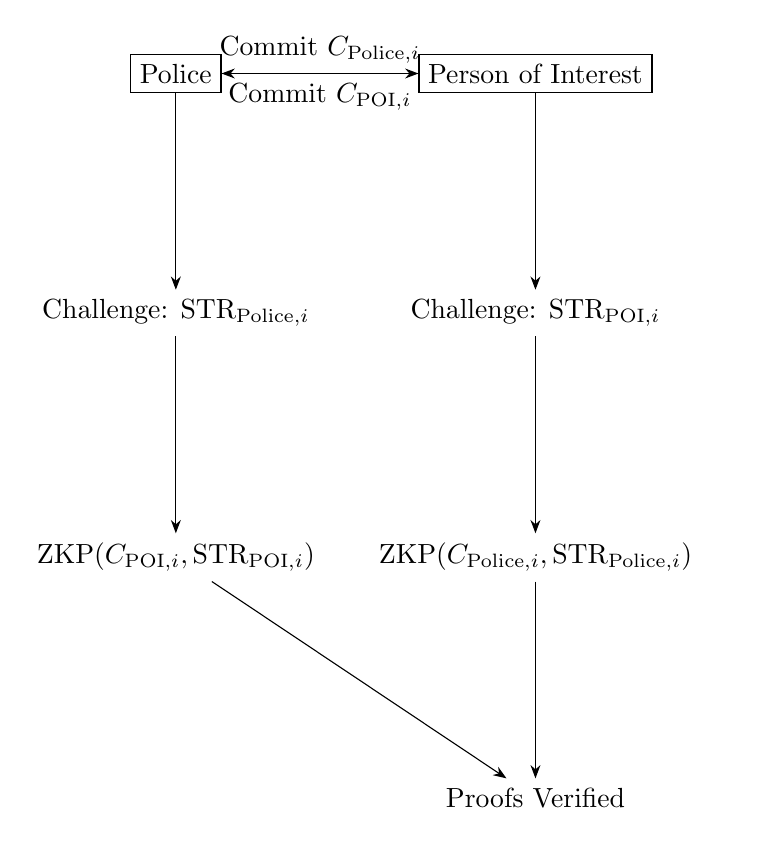
\begin{tikzpicture}[>=Stealth, node distance=2.5cm]

\node (police) [draw, rectangle] {Police};
\node (poi) [draw, rectangle, right=of police] {Person of Interest};
\node (challenge_police) [below=of police] {Challenge: STR$_{\text{Police},i}$};
\node (challenge_poi) [below=of poi] {Challenge: STR$_{\text{POI},i}$};
\node (proof_police) [below=of challenge_poi] {ZKP$(C_{\text{Police},i}, \text{STR}_{\text{Police},i})$};
\node (proof_poi) [below=of challenge_police] {ZKP$(C_{\text{POI},i}, \text{STR}_{\text{POI},i})$};
\node (verified) [below=of proof_police, text width=5cm, align=center] {Proofs Verified};

\draw[->] (police) -- (poi) node[midway, above] {Commit $C_{\text{Police},i}$};
\draw[->] (poi) -- (police) node[midway, below] {Commit $C_{\text{POI},i}$};
\draw[->] (police) -- (challenge_police);
\draw[->] (poi) -- (challenge_poi);
\draw[->] (challenge_police) -- (proof_poi);
\draw[->] (challenge_poi) -- (proof_police);
\draw[->] (proof_police) -- (verified);
\draw[->] (proof_poi) -- (verified);

\end{tikzpicture}
\end{center}

\end{document}
